\section{Recomputation of the five supplied fields}
\label{sec:experiments}
The experiments use the five fixed synthetic fields supplied with version~2. We preserve their coordinates and radii. No sensor positions were optimized to obtain the results below. The new failure-domain and budget rules are deterministic additional test models, specified before their topology is evaluated. They should not be read as measured hardware failure statistics.

\subsection{Inputs and arithmetic convention}
The field identifiers are \texttt{A\_ring\_grid\_seed3}, \texttt{B\_ring\_grid\_seed7}, \texttt{C\_poisson\_random}, \texttt{D\_hex\_dead\_zone} and \texttt{E\_two\_cluster}. Their contact counts are respectively $91,91,95,79,95$, and their common radii are $1.55,1.55,1.4,1.35,1.3$. The CSV data files are round-trip decimal exports of the original NumPy arrays. The input manifest records both original-array and CSV SHA-256 hashes, and the exports were checked to reproduce the binary64 coordinates exactly.

Every geometric Boolean decision uses exact rational arithmetic on those binary64 values. For example, the value passed as $1.3$ is its actual binary64 rational, not an unspecified real decimal with a tolerance. The circle-witness algorithm does not use a floating-point square root. The independent enclosing-circle verification also works with rational squared distances. This convention makes the reported finite result reproducible; it does not model uncertainty in field acquisition. Parameter uncertainty is treated separately by \cref{thm:stability}.

For each field we evaluate five rules:
\begin{enumerate}
\item ordinary $k$-fold coverage, for $k=1,2,3$;
\item survival of any one of four fault domains, where contact $i$ at $(x_i,y_i)$ is assigned label
\begin{equation}\label{eq:domain-assignment}
d_i=\boldsymbol1\{x_i>\operatorname{median}_j x_j\}
+2\boldsymbol1\{y_i>\operatorname{median}_j y_j\};
\end{equation}
\item a weighted deletion budget $B=3$ with $c_i=1+(i\bmod3)$, using the original zero-based contact order.
\end{enumerate}
The domain model wins when at least two distinct labels occur in the active set. The budget model wins when the active costs sum to more than three. These labels, costs and resulting facet masks are included in the result records, so the failure semantics can be reproduced independently of the plots.

\begin{figure}[!htbp]
\centering
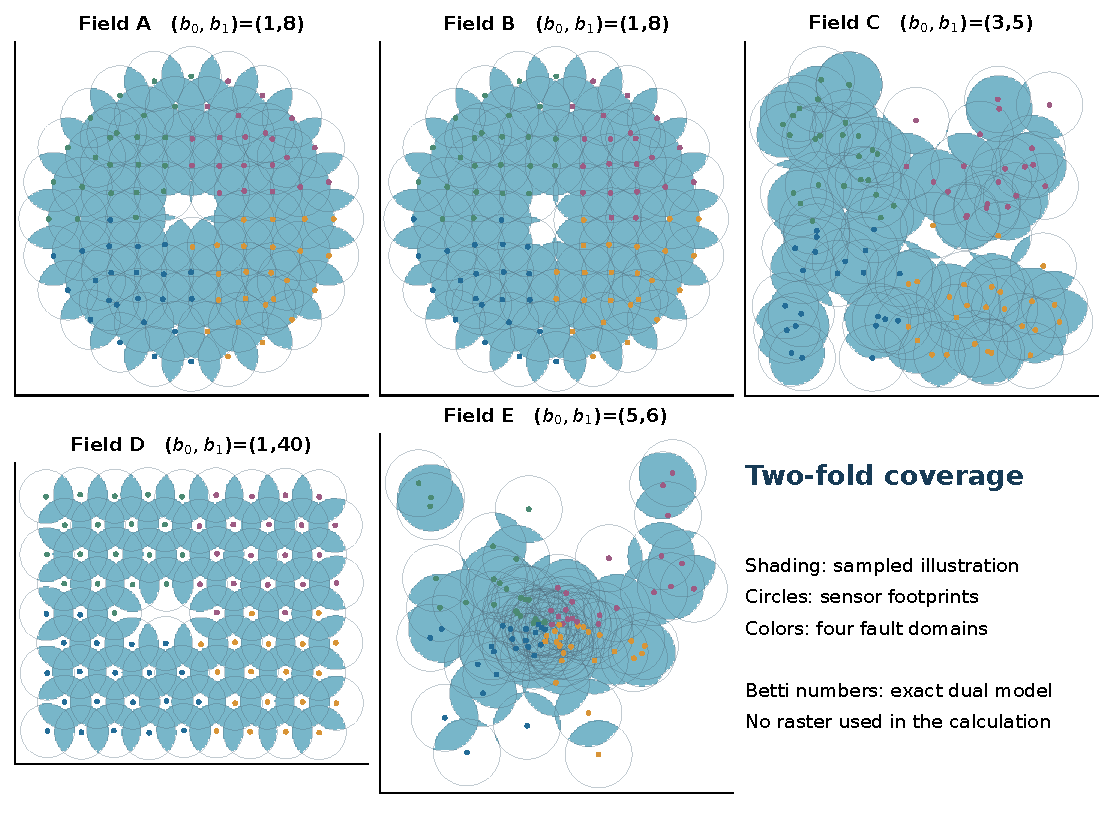
\includegraphics[width=\textwidth]{figures/five-fields.pdf}
\caption{The five fixed fields at two-fold coverage. Shading is a sampled illustration and can miss thin geometric features; it is not used to determine topology. The displayed Betti numbers come from the complete exact dual two-skeleton. Contact colors show the four deterministic domains in \cref{eq:domain-assignment}.}
\label{fig:fields}
\end{figure}
\FloatBarrier
\clearpage

\subsection{Complete dual counts}
\begin{longtable}{llrrrrrr}
\caption{Complete dual two-skeleton counts and Betti numbers. The domain model survives every loss of one of the four stated domains.}\label{tab:all-results}\\
\toprule Field & Rule & $V$ & $E$ & $T$ & $\rank\partial_2$ & $b_0$ & $b_1$ \\ \midrule\endfirsthead
\toprule Field & Rule & $V$ & $E$ & $T$ & $\rank\partial_2$ & $b_0$ & $b_1$ \\ \midrule\endhead
\bottomrule\endfoot
A & $k=1$ & 153 & 1821 & 8798 & 1668 & 1 & 1 \\
A & $k=2$ & 153 & 1037 & 2498 & 877 & 1 & 8 \\
A & $k=3$ & 153 & 533 & 615 & 342 & 4 & 42 \\
A & Domains & 45 & 100 & 84 & 59 & 4 & 0 \\
A & Budget & 153 & 854 & 1741 & 682 & 1 & 20 \\
\addlinespace
B & $k=1$ & 150 & 1753 & 8223 & 1603 & 1 & 1 \\
B & $k=2$ & 150 & 990 & 2263 & 833 & 1 & 8 \\
B & $k=3$ & 150 & 522 & 585 & 332 & 4 & 44 \\
B & Domains & 46 & 109 & 111 & 67 & 4 & 0 \\
B & Budget & 150 & 837 & 1710 & 667 & 1 & 21 \\
\addlinespace
C & $k=1$ & 107 & 987 & 3869 & 878 & 1 & 3 \\
C & $k=2$ & 107 & 678 & 1822 & 569 & 3 & 5 \\
C & $k=3$ & 105 & 456 & 842 & 343 & 4 & 12 \\
C & Domains & 38 & 126 & 209 & 89 & 1 & 0 \\
C & Budget & 107 & 589 & 1483 & 475 & 3 & 10 \\
\addlinespace
D & $k=1$ & 118 & 563 & 848 & 445 & 1 & 1 \\
D & $k=2$ & 118 & 157 & 0 & 0 & 1 & 40 \\
D & $k=3$ & 118 & 0 & 0 & 0 & 118 & 0 \\
D & Domains & 27 & 23 & 0 & 0 & 4 & 0 \\
D & Budget & 118 & 110 & 0 & 0 & 22 & 14 \\
\addlinespace
E & $k=1$ & 130 & 4617 & 107292 & 4488 & 2 & 1 \\
E & $k=2$ & 130 & 4214 & 94985 & 4083 & 5 & 6 \\
E & $k=3$ & 128 & 3910 & 85522 & 3795 & 16 & 3 \\
E & Domains & 104 & 3507 & 77706 & 3404 & 1 & 0 \\
E & Budget & 128 & 4120 & 90824 & 3994 & 6 & 4 \\
\addlinespace
\end{longtable}

All $25$ model computations use the same maximal nerve faces within their respective field. Only the winning test changes. The ring fields have identical two-fold Betti pairs $(1,8)$ but different higher-order and weighted results. The random field gives $(3,5)$ at two-fold coverage, illustrating that its topology cannot be established by a coarse raster comparison alone. Field~D has $118$ isolated three-fold components and no dual three-fold edges, whereas its two-fold graph has $157$ edges and no triangles, giving $40$ independent graph cycles.

The structured rules change the region in ways that a single overlap threshold does not capture. In Field~E, two-fold coverage gives $(5,6)$; survival of a complete domain loss gives $(1,0)$; the chosen weighted budget gives $(6,4)$. The domain-surviving region is a subset of the two-fold region, but removing parts of a region can delete whole components as well as remove or create holes. There is no monotonicity law for either Betti number separately under set inclusion.

\begin{figure}[!htbp]
\centering
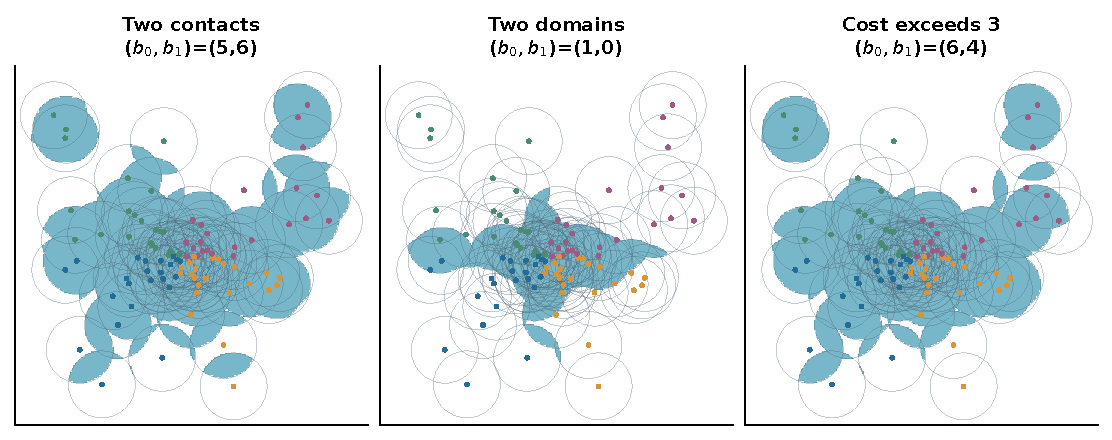
\includegraphics[width=\textwidth]{figures/structured-field-E.pdf}
\caption{Field~E under three distinct failure rules. Geometric shading is illustrative; exact counts are in \cref{tab:all-results}. Domain redundancy requires contacts from different groups, whereas the budget rule evaluates their stated deletion costs. None of these panels certifies coverage of an unstated external target.}
\label{fig:structured}
\end{figure}

\subsection{Completion and correction of the dense example}
The equal-radius nerve of Field~E has $95$ vertices, $1810$ edges and $24\,956$ triangles. An independent recount of the two-fold coalition shadow gives
\[
\abs{\Delta_2^{(0)}}=1810,\qquad
\abs{\Delta_2^{(1)}}=836\,991.
\]
Thus the number previously described as its vertex count is an edge count. This revision corrects the abstract, discussion and size comparison rather than carrying that description forward.

There are $130$ maximal nerve faces in the exact facet list. All $130$ win for two-fold coverage. In the dual complex the graph has $4214$ edges and five components, so its cycle-space dimension is
\[
4214-130+5=4089.
\]
The full list of $94\,985$ triangle columns has rank $4083$. It follows that
\[
b_1=4089-4083=6.
\]
The duality theorem transfers this finite calculation to the two-fold covered region. The calculation completes this one previously unfinished case. It is not a claim to resolve an unrelated open conjecture.

\begin{figure}[!htbp]
\centering
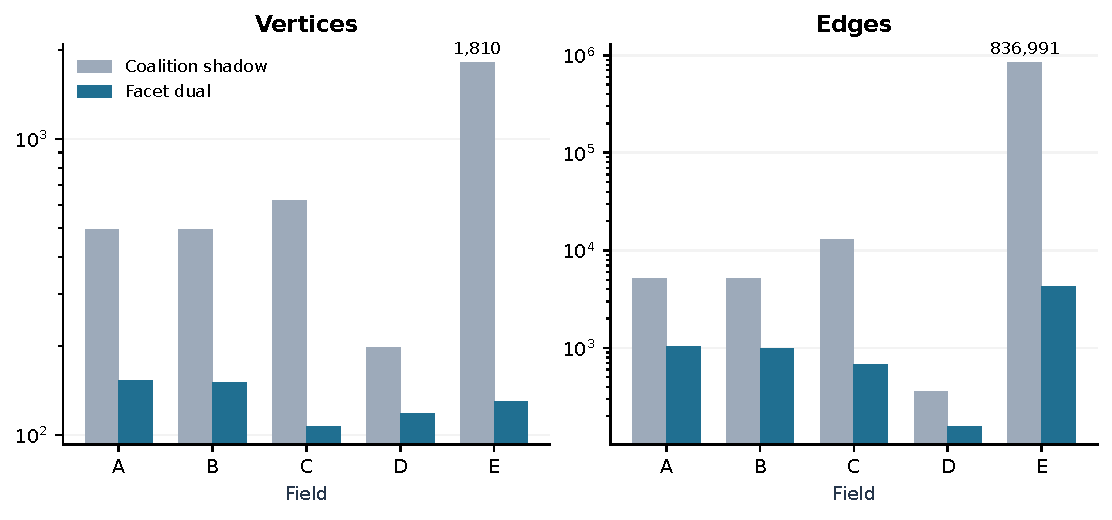
\includegraphics[width=\textwidth]{figures/compression.pdf}
\caption{Exact counts in the coalition-shadow and facet-dual representations for two-fold coverage. The vertical axes are logarithmic. The dual need not be smaller on every input, and these empirical reductions are not a universal linear-size theorem. The dense-field shadow has $1810$ vertices and $836\,991$ edges.}
\label{fig:compression}
\end{figure}
\FloatBarrier

\subsection{Independent checks and their scope}
The geometry audit compares every disk pair and triple with the facet face oracle: $125\,580$ tests in each ring field, $142\,880$ in each of Fields~C and~E, and $82\,160$ in Field~D, totaling $619\,080$ comparisons. There is no exact pair or triple tangency in these fixed fields. The audit additionally checks each returned facet using the equal-radius Helly criterion and checks that adjoining any absent contact destroys the face property. Field~E's ordinary pair and triple counts independently reproduce $1810$ and $24\,956$.

The two-fold boundary rank is recomputed with a separate set-column elimination that uses the smallest available pivot. The main routine uses integer bit columns with the largest available pivot. Both orders give ranks $877,833,569,0,4083$ for Fields~A--E. This is an independent arithmetic implementation of the rank check, not an independent proof-assistant formalization.

The control suite contains ten tests. Its exhaustive small geometric controls compare all nonempty subsets in $50$ seven-contact equal-radius fields with a different minimum-enclosing-circle oracle. Its combinatorial controls compare the dual and minimal-coalition models on $150$ random small nerves under four types of monotone rule, giving $600$ comparisons of $(b_0,b_1)$. Additional controls address exact tangency, a one-unit binary64 separation beyond tangency, unequal and coincident disks, zero radii, very small and very large power-of-two scales, radical signs, budget validation, correlated-domain failure and the continuous triangle certificate.

The geometric and combinatorial control tests are evidence about the implementation. The all-input assertions are established by the mathematical proofs, not by extrapolating the controls. In particular, matching all pair and triple tests would not by itself establish completeness of an arbitrary facet enumeration; \cref{thm:witness} supplies that missing logical guarantee.

\subsection{Reproducibility and limitations}
The repository contains the CSV inputs, radii, exact facet masks, all $25$ model counts, the separate geometric and rank audit, the corrected shadow edge recount and the figure generator. The main geometry and homology computations use Python's standard library; the figure generator additionally uses NumPy and Matplotlib. Figures are generated from the saved results and input coordinates. Rasterization occurs only in the illustrations.

The experiment does not compare performance against every existing multicover implementation, determine a practical optimal failure model or establish superiority over the bifiltration methods of~\cite{corbet,alonso}. Its purpose is a reproducible evaluation of the stated construction and a finite completion of the dense v2 example. Runtime observations depend on implementation and machine and are not used as asymptotic claims.

The current package does not provide a Lean formalization. Its exact computations concern $H_0$ and $H_1$ over $\FF$; they do not assert integral homology, all higher Betti numbers or clinical reliability. The target certificate is proved for closed planar triangles with the stated metric. A curved-surface implementation requires certified metric error bounds or another geometric certificate, as emphasized in the companion archive~\cite{ecog}.
\FloatBarrier
